\documentclass[11 pt,oneside]{article}
\usepackage[spanish]{babel}
\usepackage{hyperref}
\usepackage{fancyhdr}
\hypersetup{urlcolor=blue, colorlinks=true}
\usepackage{caption}
\usepackage{subcaption}
\usepackage{float}
\usepackage{rotating}

%\usepackage{mwe}
%\usepackage[latin1]{inputenc} % acentos sin codigo
%\usepackage{enumerate} % enumerados
\pagestyle{plain} 

\usepackage{graphicx}
  % declare the path(s) where your graphic files are
   \graphicspath{{./figuras/}}
  % and their extensions so you won't have to specify these with
  % every instance of \includegraphics
   \DeclareGraphicsExtensions{.pdf,.jpeg,.png}
   
   \pagenumbering{arabic}

\usepackage{vmargin}

\setpapersize{A4}
\setmargins{2.5cm}       % margen izquierdo
{1cm}                        % margen superior
{16.5cm}                      % anchura del texto
{23.42cm}                    % altura del texto
{10pt}                           % altura de los encabezados
{1cm}                           % espacio entre el texto y los encabezados
{0pt}                             % altura del pie de página
{2cm}                           % espacio entre el texto y el pie de página

%%%% SECTION WITHOUT NUMBER %%%%%%%%%%%%%%%%%
\makeatletter
% we use \prefix@<level> only if it is defined
\renewcommand{\@seccntformat}[1]{%
  \ifcsname prefix@#1\endcsname
    \csname prefix@#1\endcsname
  \else
    \csname the#1\endcsname\quad
  \fi}
% define \prefix@section
\newcommand\prefix@section{}
\makeatother

\renewcommand{\thesubsection}{\alph{subsection}}


\begin{document}

.\\
Autor: Alvaro Camacho Mora\\
Profesor: Dr. Daniel Herrera C.\\
III-C 2018\\
Procesamiento Digital de Im\'agenes\\
Tarea 5
\\

La figura 1 muestra la tendencia mostrada por laimplementaci\'on del filtro en esl espacio. En color rojo se muestra el filtro separable, mientras que en azul se tiene el filtro 2D. Cabe destacar que el filtro separable tiene una tendencia esperada, donde aumenta el tiempo de ejecucion al aumentar el tama\~no del kernel. En el caso del filtro 2D, la tendencia no es la esperada y es quizas por el hecho que la implementaci\'on en OpenCV tiene optimizaciones que a cierto tama\~no de kernel se pasa a la frecuencia lo que incide directamente en esos cambios de tiempo de ejecuci\'on.\\

La figura 2 muestra el caso de la implementaci\'on de ambos filtros en el dominio de la frecuencia. En rojo se muestra el resultado de aplicar el filtro separable donde es evidente que por tener que aplicar dos veces el kernel en la frecuencia se tiene un tiempo de ejecucion mayor. En azul es la respuesta del filtro 2D, donde el tiempo de ejecuci\'on es menor y tiene una tendencia esperada, es decir, se estabiliza.\\

La figura 3 y 4 muestran la comparacion de la implementaci\'on del filtro 2D y separable 2D, respectivamente. Se muestra en la figura 3 que la implementaci\'on en la frecuencia se vuelve mas eficiente cuando el Kernel es aproximadamente mayor a 60. Tambi\'en se observa como cuando el tama\~no del kernel es grande la funci\'on de OpenCV utiliza el procesamiento en la frecuencia y ambas curvas casi que se traslapan. En el caso de la figura 4 el punto de quiebre se da cuando el kernel es mayor a 115 aproximadamente. \\

La figura 5 muestra todas las implementaciones en un solo cuadro, donde es evidente que la implementaci\'on separable en el tiempo es m\'as eficiente hasta cierto tama\~no de kernel (53 aproximadamente), mientras la implementacio\'on en la frecuencia del filtro separable nunca esta tendiendo a ser mas eficiente.
\begin{figure}[H]
\centering
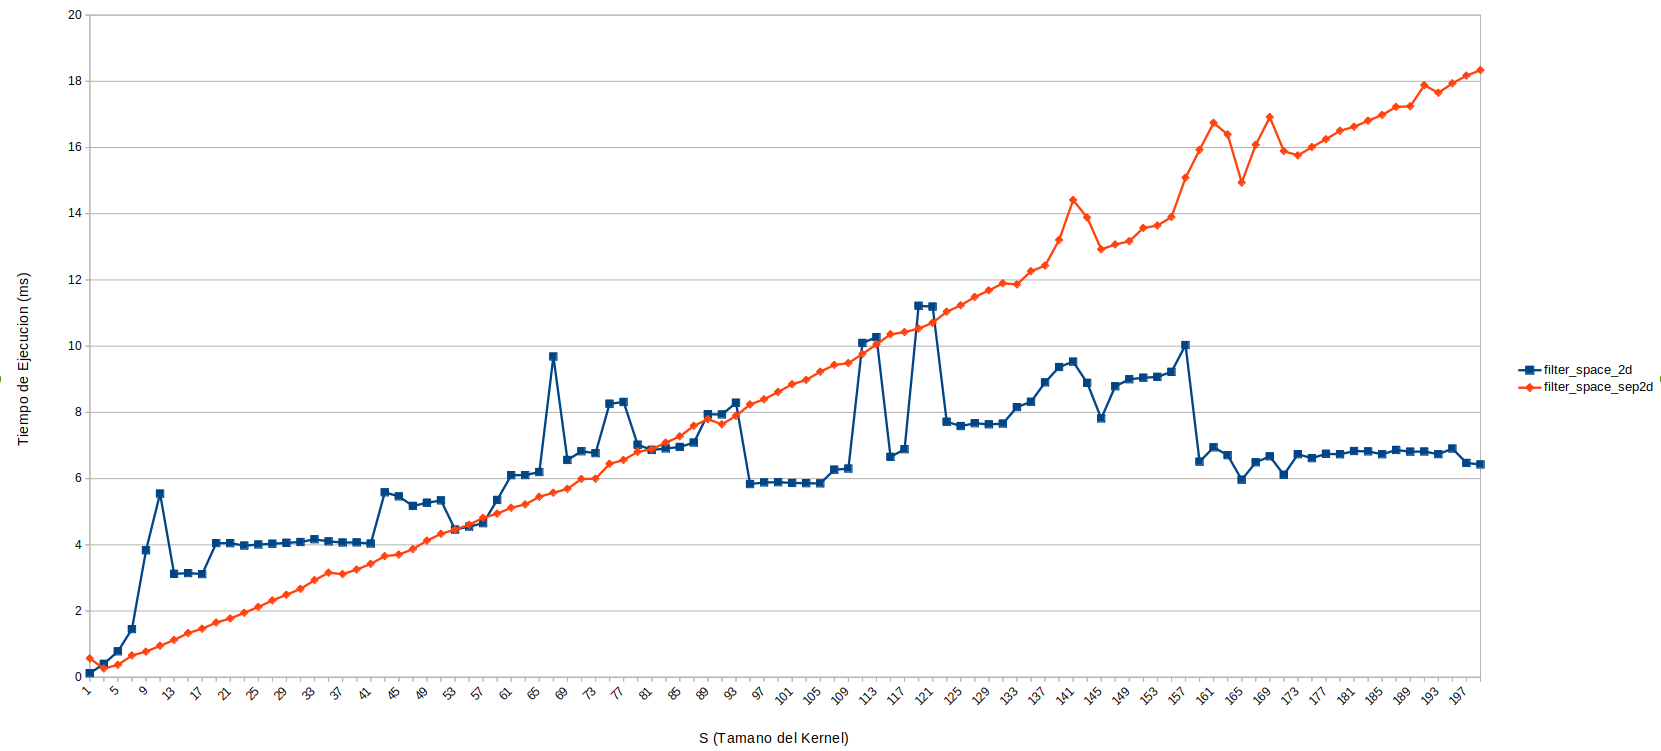
\includegraphics[width=17cm]{espacio}
\caption{Muestra la tendencia de aplicar el kernel 2D y separable en el espacio} \label{fig:2d}
\end{figure} 

\begin{figure}[H]
\centering
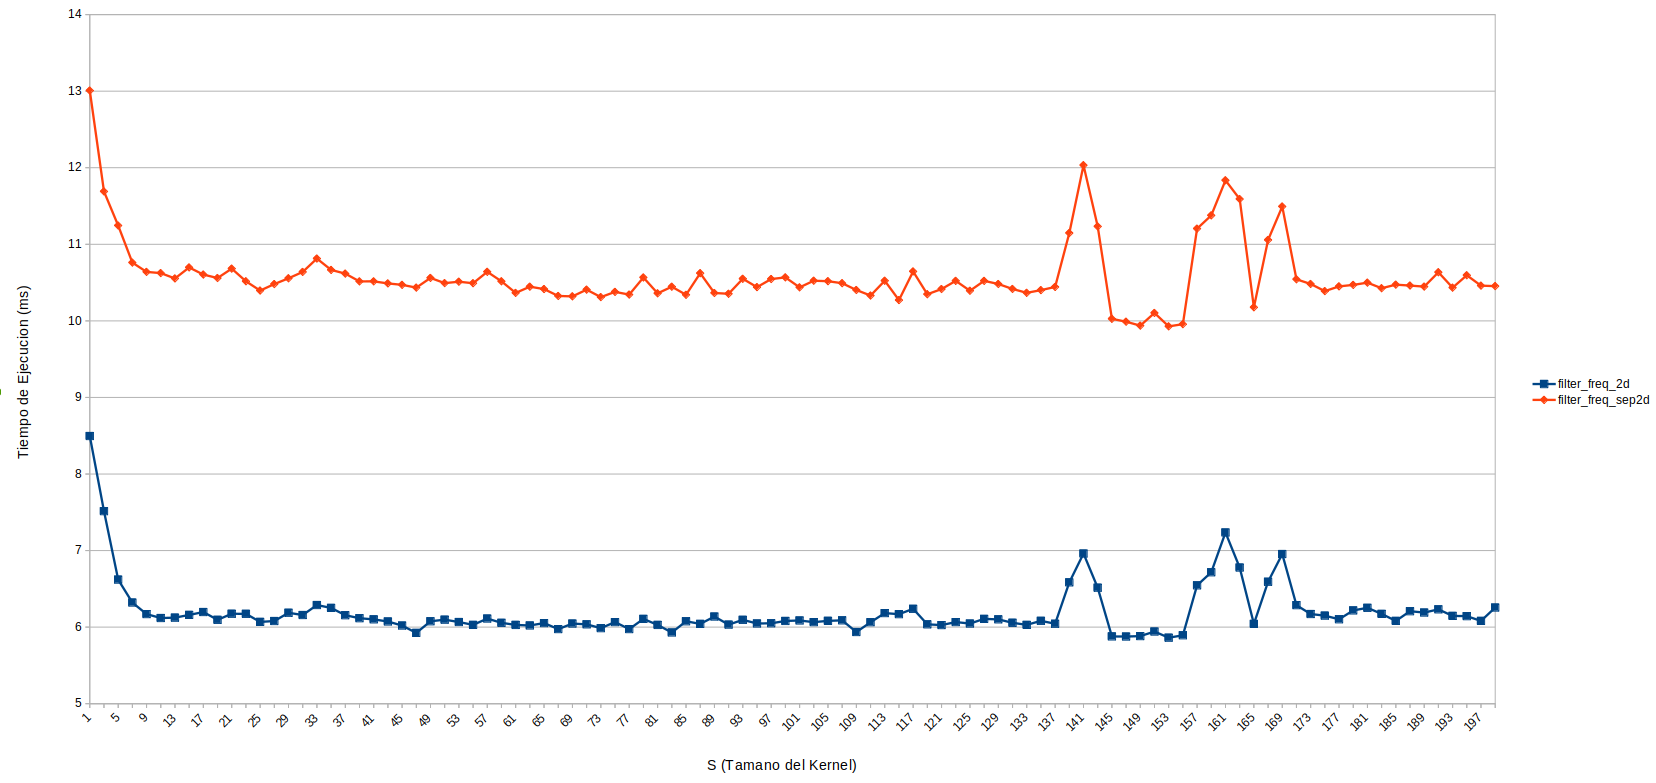
\includegraphics[width=17cm]{freq}
\caption{Muestra la tendencia de aplicar el kernel 2D y separable en la frecuencia} \label{fig:2d}
\end{figure} 

\begin{figure}[H]
\centering
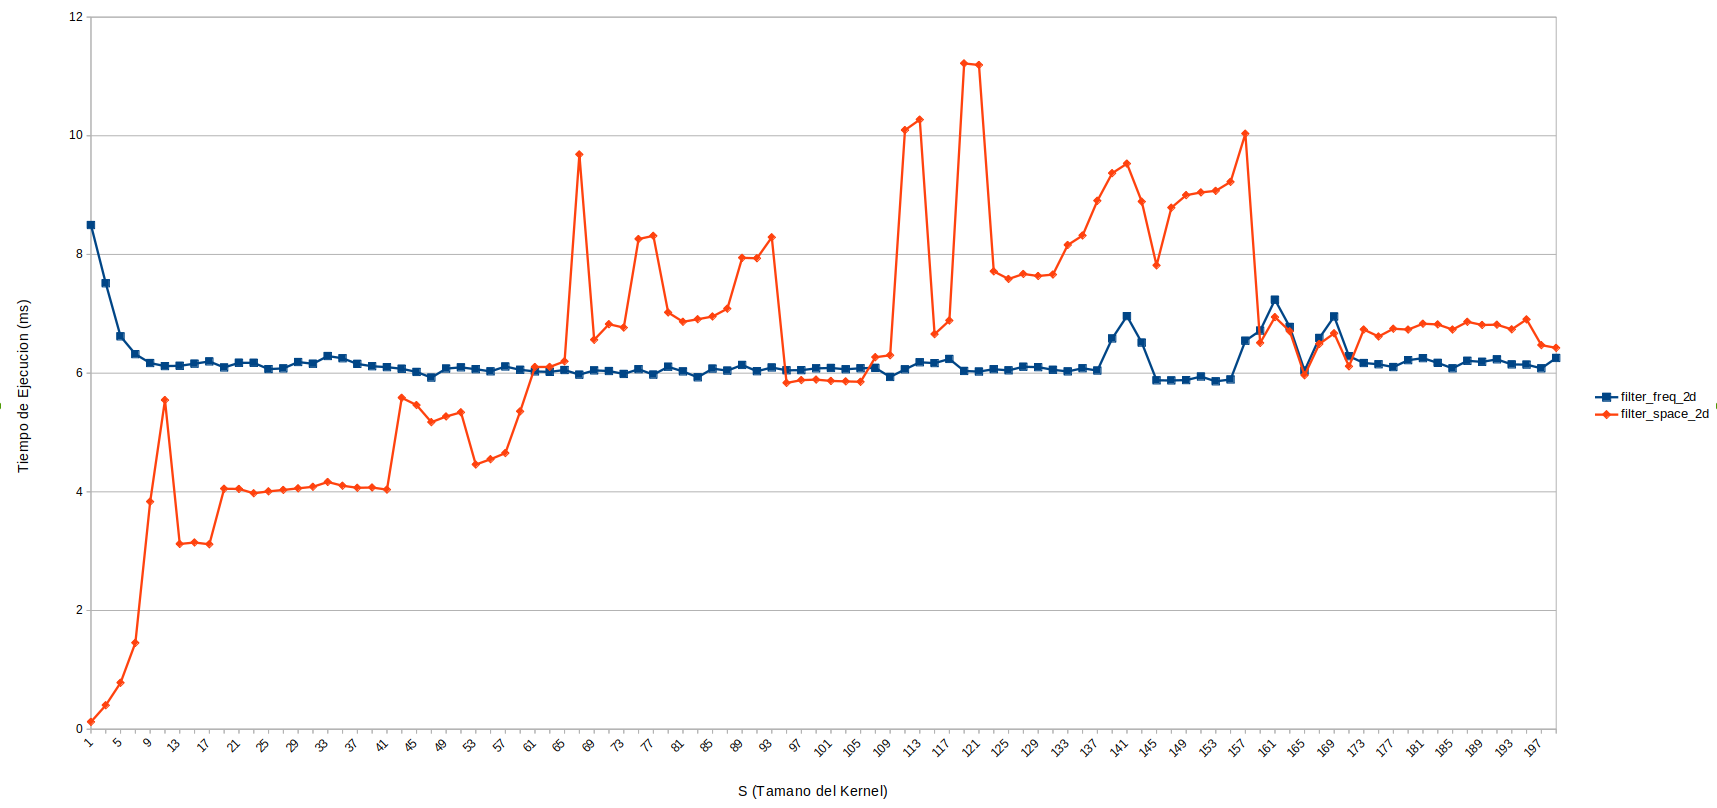
\includegraphics[width=17cm]{2d}
\caption{Muestra la tendencia de kernel 2D en el espacio y frecuencia} \label{fig:2d}
\end{figure} 

\begin{figure}[H]
\centering
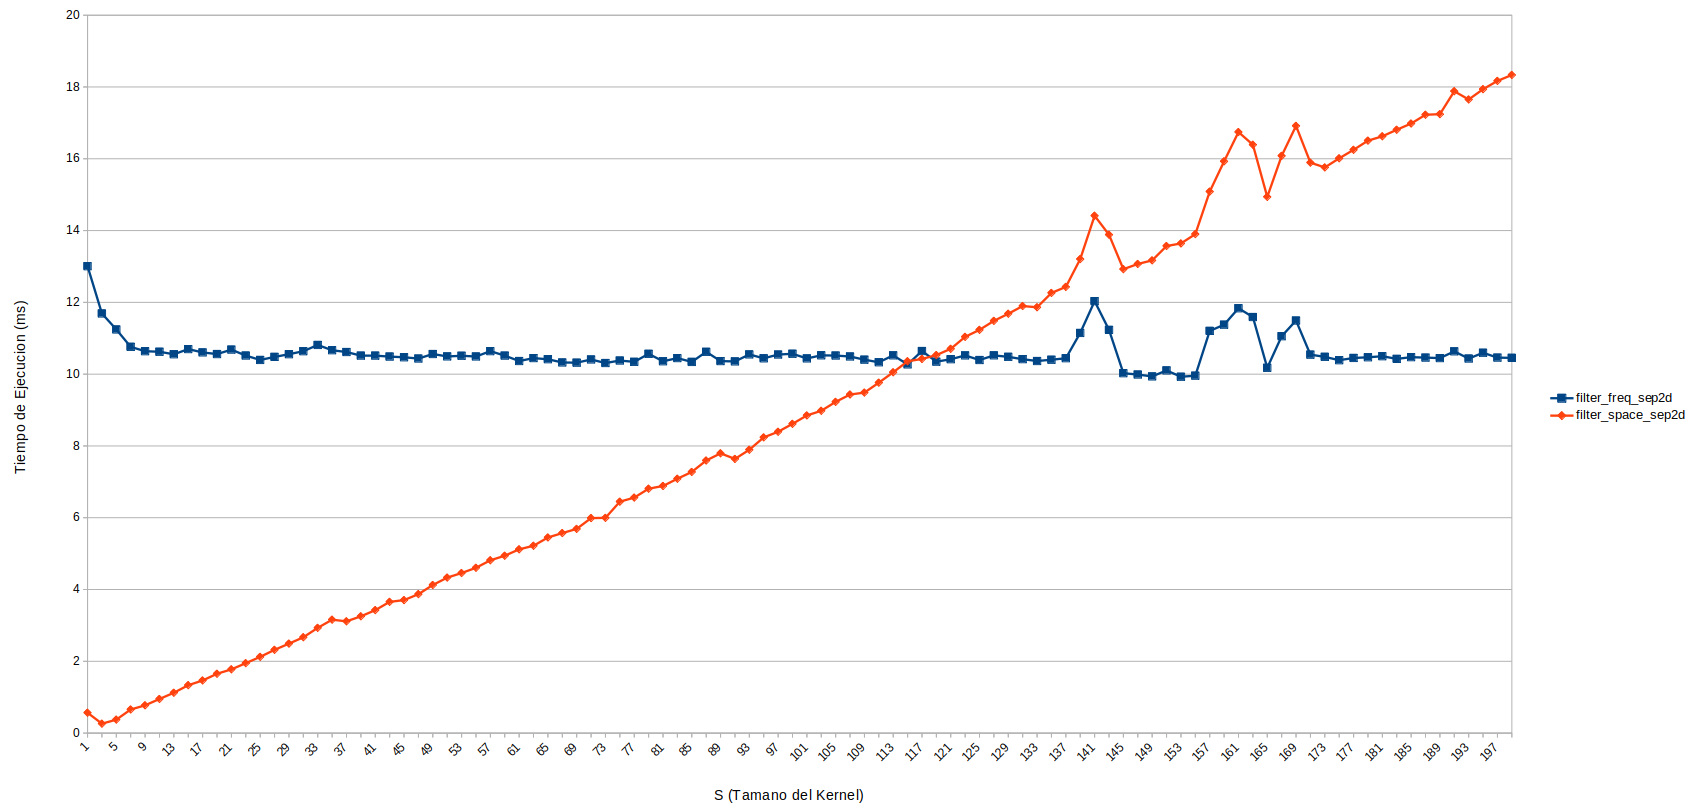
\includegraphics[width=17cm]{sep}
\caption{Muestra la tendencia de kernel 2D separable en el espacio y frecuencia} \label{fig:2d}
\end{figure} 

\begin{figure}[H]
\centering
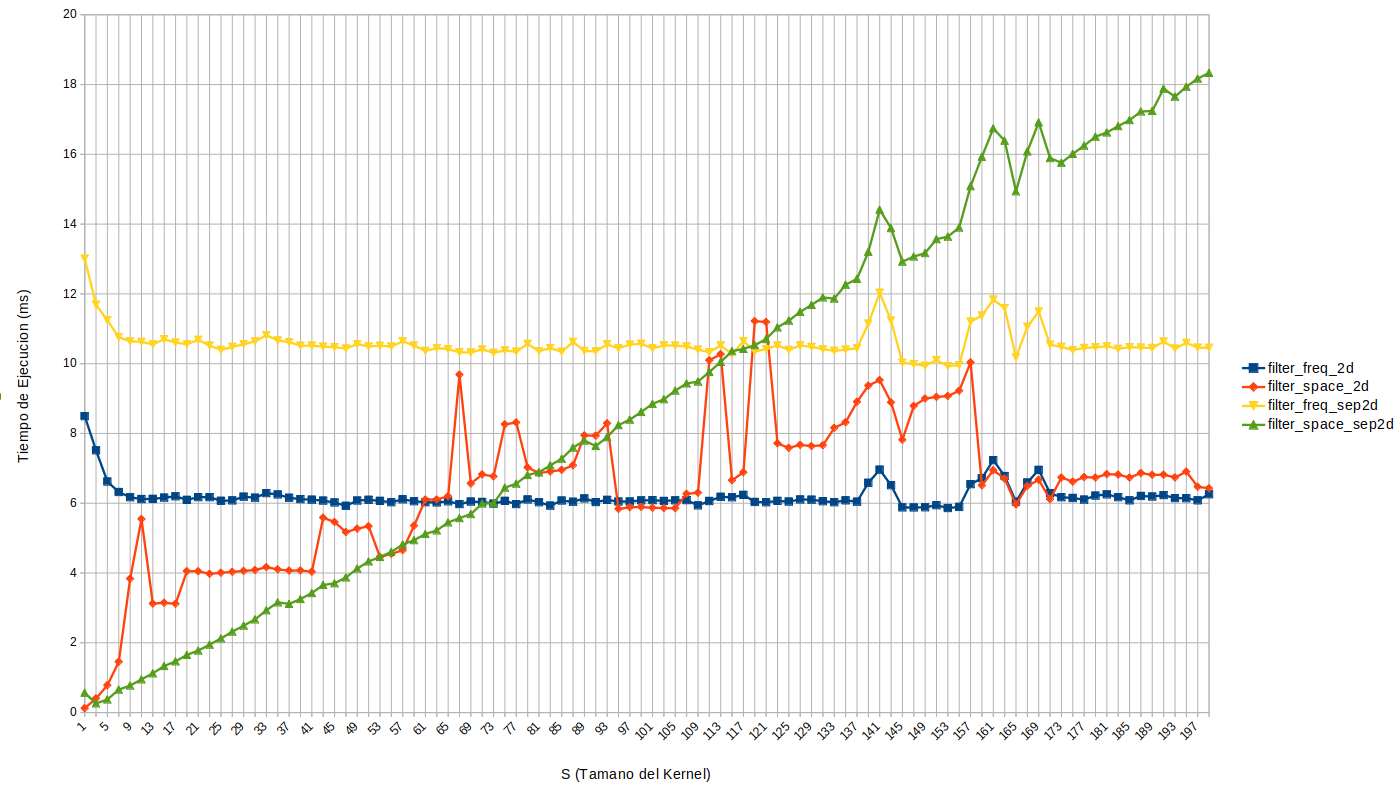
\includegraphics[width=17cm]{todos}
\caption{Muestra todas las implementaciones hechas} \label{fig:2d}
\end{figure} 

\clearpage



\end{document}
